\section{Identification of jets from bottom quarks}
Accurately identifying jets from bottom quarks is a crucial part of physics program involving top quarks and the Higgs boson. The relatively large lifetime, hadronization properties of the bottom quark and the possible semileptonic decays of b hadrons allow us to experimentally identify the jets that arise from bottom and charm quarks through the technique of flavor tagging. The idea of flavor tagging is to use discriminating variables to distinguish between jets from bottom, charm and light quarks on a statistical basis by assigning a discriminator value for jets that is on average higher for jets arising from bottom quarks than for the ones arising from light quarks. Jets that pass a certain pre-determined threshold of the discriminator value are taken to be tagged as a certain flavor. In the following section, we will give an overview of flavor tagging at CMS, with a specific focus on the development and re-optimization of the Combined Multivariate (cMVAv2) b tagging algorithm for Run II.

\subsection{Discriminating variables}
The most important discriminating variables for flavor tagging are the kinematic properties of jets and leptons, as well as the existence and properties of tracks from charged particles and vertices associated to either the primary hard interaction in the proton-proton collision or the secondary vertices from the decay of b or c hadrons. The secondary vertex of b hadron decay, which is displaced with respect to the primary vertex due to the long life time of b hadrons, is an expecially salient feature of b hadron decays that the b tagging algorithms seek to exploit through accurate track and vertex reconstruction. 

The tracks reconstructed by the inner tracking detector and associated to jets are used for b tagging only in case they are of sufficient quality, i.e. they pass the track selection. This means they must have a transverse momentum of at least~1~GeV, a normalized~$\chi^2$~quality parameter for the fit to hits below~5 and at least~8 hits in the tracker with at least 2 in the inner pixel detector. Furthermore, the impact parameter~(IP), which is defined as the distance of closest approach between the primary vertex and the track trajectory is required to be less than~0.2~(17)~cm in the transverse (longitudinal) direction to ensure that the tracks are sufficiently close to the primary vertex and thus reduce the contribution from pileup. The distance of closest approach between the jet and the track must be smaller than~0.07~cm and the decay length, defined as the distance between the primary vertex and the point of closest approach between the track and the jet must be less than~5~cm~\cite{CMS-PAS-BTV-15-001}.

\subsection{Vertex reconstruction}
Tracks passing this selection are used for vertex reconstruction in the adaptive vertex reconstruction (AVR) algorithm~\cite{}. Vertices reconstructed by AVR must pass further selection criteria designed to suppress vertices that are unlikely to originate from b hadron decay. These selection criteria require a vertex to have sufficient unique tracks, a flight distance that is significant and a mass of less than~6.5~GeV and incompatible with the $K_S^0$ hadron. The requirements are described in detail in~\cite{CMS-PAS-BTV-15-001}.

An alternative to AVR, where tracks are required to be associated to jets and therefore vertex reconstruction is seeded by jets, is the inclusive vertex finder (IVF) algorithm~\cite{}. As the name implies, the IVF algorithm starts with the set of all tracks in the event that pass somewhat looser selection criteria than used for AVR. Vertices are found by fitting all tracks simultaneously using an adaptive fitting algorithm looking for clusters. A further arbitration step assigns tracks to either the primary or secondary vertex based on compatibility and pixel hits, or removes secondary vertices of low quality. The IVF algorithm reconstructs about~10~\%~(15~\%)~more often the vertices from bottom (charm) hadrons, but also increases the fraction of vertices reconstructed for light jets by about~8~\%. The overlap between the two algorithms is about~60\%, meaning that both vertex fitters provide some independent information on the event.

\subsection{Combining information}
Using machine learning, signals from various regions of the detector can be combined effectively to develop a discriminator between b jets and light jets. Such techniques are especially suited to exploit sources of information that are partially correlated, such as the AVR and IVF vertices. The cMVAv2 b tagging algorithm combines the output of different low and high level b tagging algorithms, developed independently and using partially correlated variables, into a single high level discriminator. Before we can describe the cMVAv2 in detail, we must therefore discuss the different b tagging algorithms used at CMS.

The Jet Probability (JP) tagger~\cite{Chatrchyan:2012jua} was developed during Run I and is a simple multivariate likelihood discriminator based on track properties. In JP, the likelihood for a jet to originate from the primary vertex, as opposed to a secondary vertex, is computed by multiplying the per-track likelihoods, based on the track impact parameter and detector resolution. In a version of the JP tagger, the 4 tracks that have the highest IP significance ($\mathrm{IP} / \sigma_{\mathrm{IP}}$) are given a higher weight such that the new tagger, denoted Jet B-Probability (JBP) is more efficient in discriminating against b jets.

The semileptonic decays of the b hadron to muons through $\mathrm{b} \rightarrow \mathrm{\mu}^- \bar{\nu}_{\mathrm{\mu}} s$, which happens with a branching fraction of about~$20\%$, makes it possible to use the presence of a reconstructed muon in a jet for b tagging. The Soft Muon (SM) algorithm in CMS relies on the presence of a muon in the jet constituents, but not on the presence of a secondary vertex. Similarly, the decay of a b hadron to an electron is exploited through the Soft Electron (SE) tagger~\cite{CMS-PAS-BTV-15-001}. 

The Combined Secondary Vertex algorithm V2 (CSVv2), based on the original CSV implementation introduced in Run I~\cref{Chatrchyan:2012jua}, uses machine learning to combine track and secondary vertex information such as vertex mass or flight distance. Based on the presence and quality of the secondary vertex, the CSVv2 is optimized in several categories, with either a good secondary vertex, in which case the flight distance and other vertex related variables are defined, the pseudo-vertex category with two good tracks but no vertex fit, in which case the track parameters are used, and a no vertex category that uses information only from displaced tracks. The final CSVv2 discriminant is a likelihood that is a combination of binary classifiers in all 3 categories based on artificial neural networks with a single hidden layer. The CSVv2 algorithm has been deployed on both the AVR vertices as CSVv2 (AVR) and the IVF vertices, denoted CSVv2 (IVF). The CSVv2 (IVF) has an efficiency of about~$66\%$ for b jets at a mistag rate for light jets (udsg-associated) of about~$1\%$ based on~\ttbar~simulation at the CSVv2 medium working point~\cite{CMS-PAS-BTV-15-001}.

\subsection{The Combined Multivariate tagger: cMVAv2}
In Run II, we have developed an improved b tagger algorithm for CMS that combines the aforementioned individual b taggers, relying on various sources of information, to a single discriminator using boosted decision trees via the scikit-learn package. This combined discriminator, denoted cMVAv2, exploits the fact that the AVR and IVF vertex reconstruction algorithms may reconstruct independent vertices, the presence or lack of soft leptons and secondary vertex information simultaneously. The tagger is optimized on~\ttbar~simulation, with cross-validation on a multijet simulation sample. At a similar b-jet efficiency to the CSVv2 medium working point, the cMVAv2 b-tagger algorithm reduces the mistag rate for light jets from $1\%$ to about $0.5\%$, as seen on~\cref{fig:btag_roc}.

\begin{figure}
\begin{centering}
\subfloat[The b tagging and mistagging efficiency.]{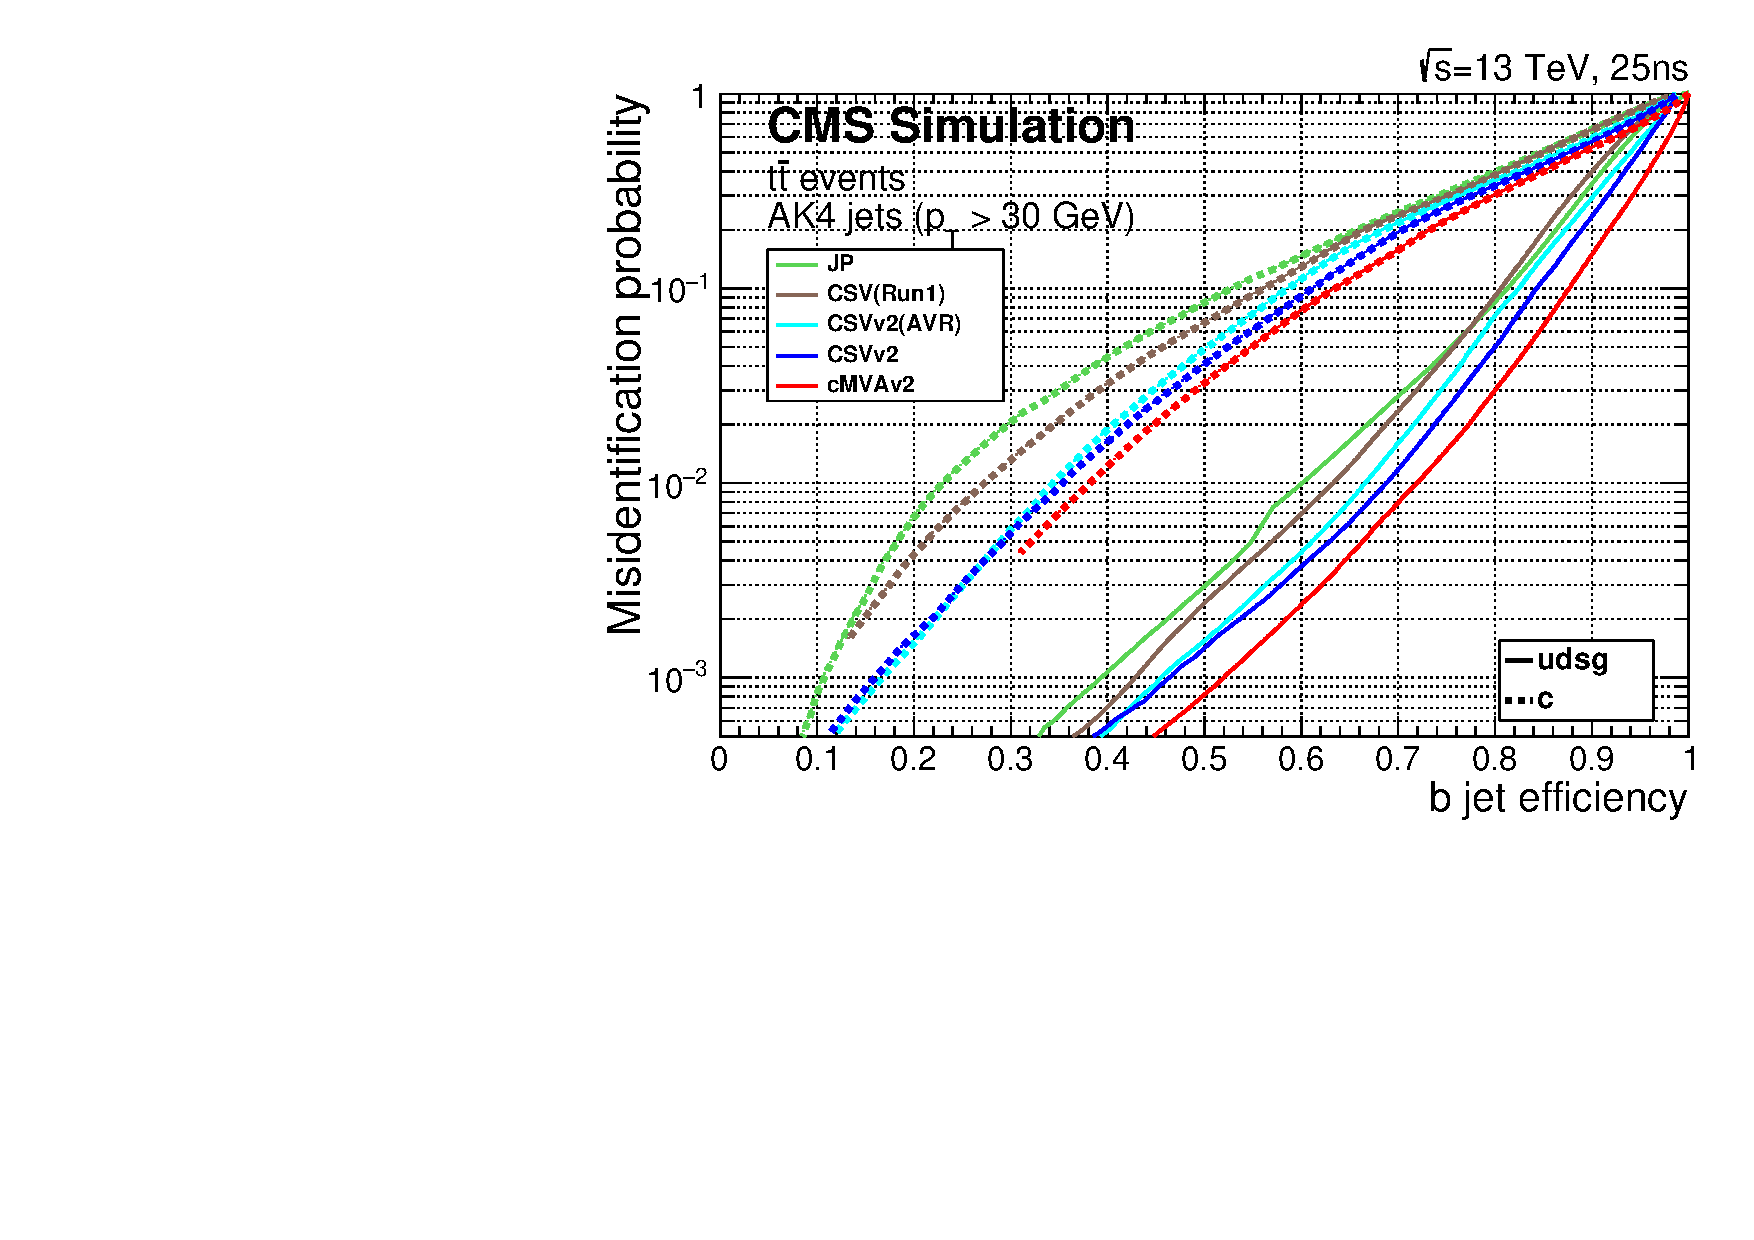
\includegraphics[width=0.5\textwidth]{figures/btv/Figure_008.pdf}}
\subfloat[The discriminant distribution of cMVAv2.]{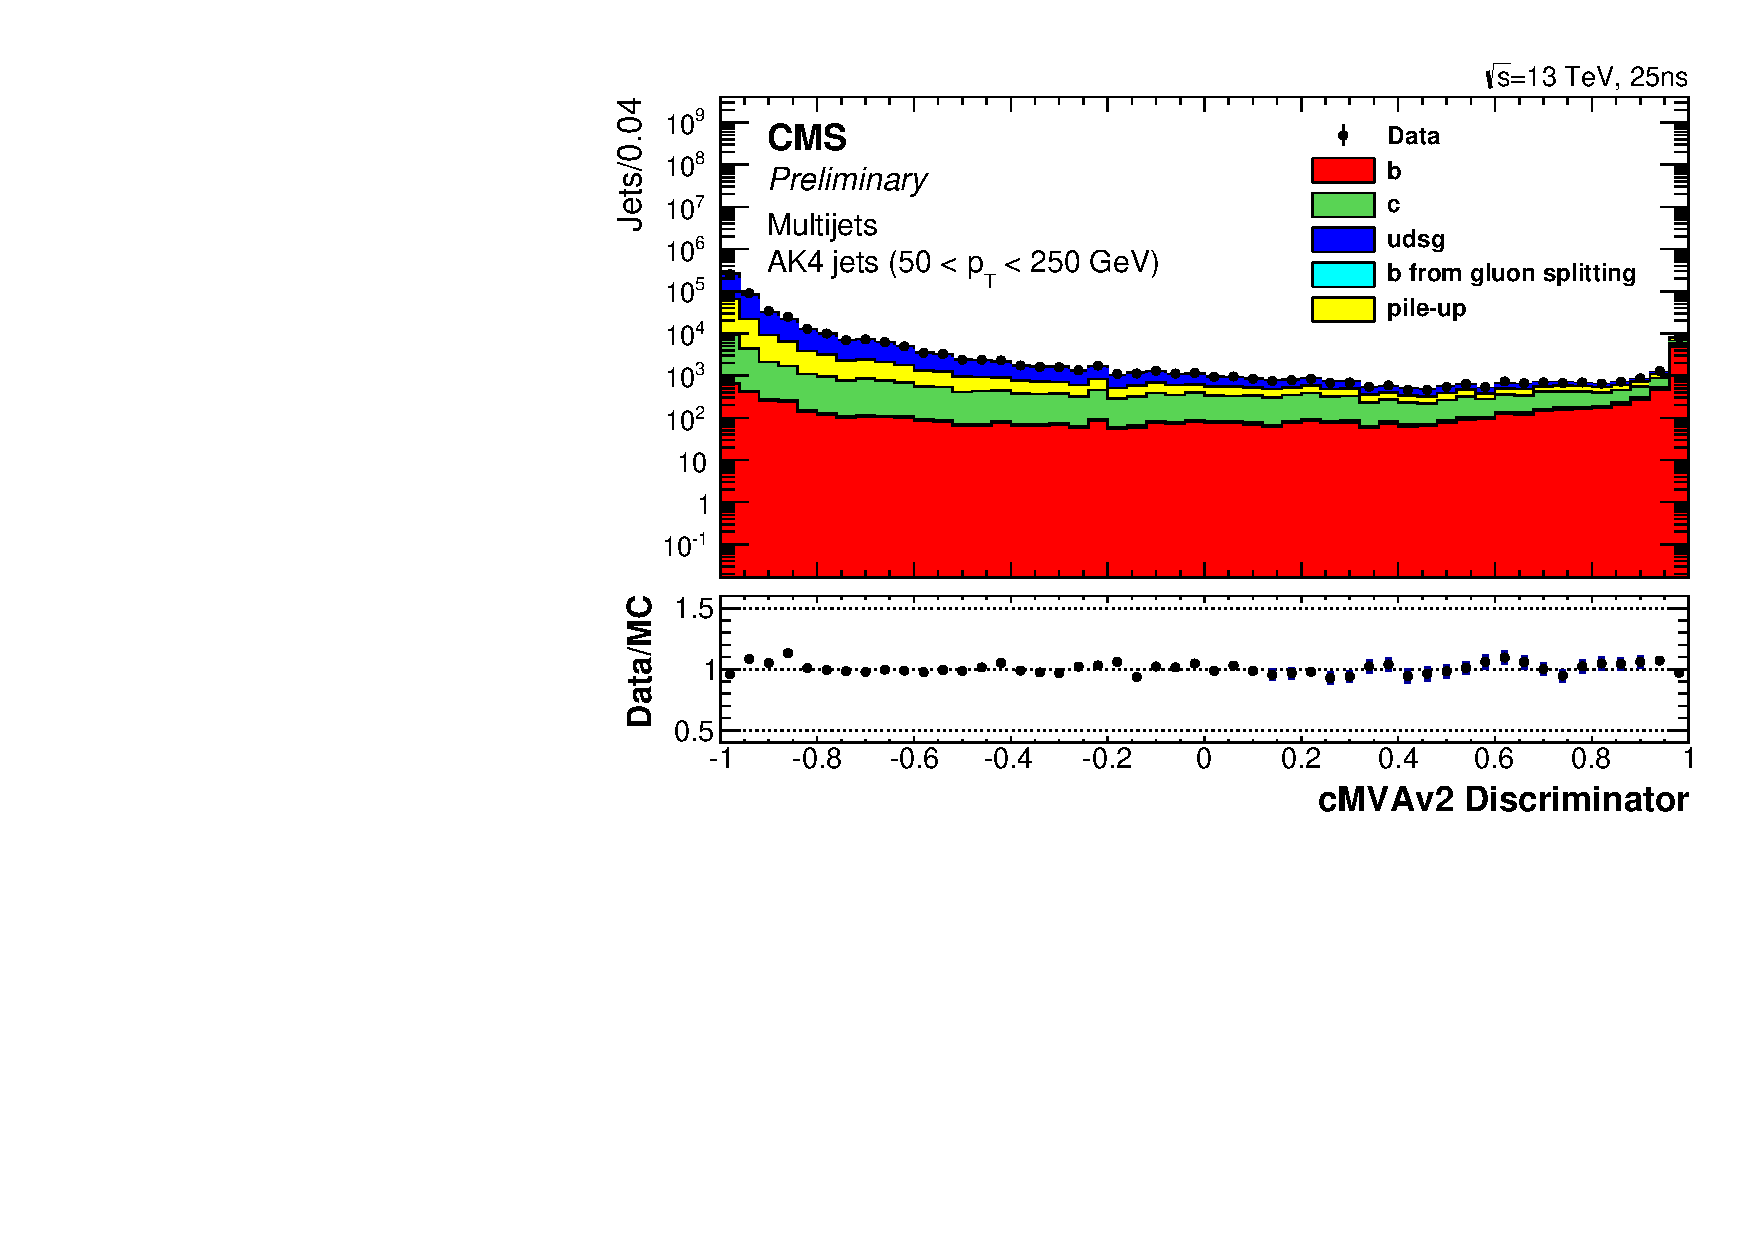
\includegraphics[width=0.5\textwidth]{figures/btv/Figure_007-a.pdf}} \\
\caption{The performance of the CMS b taggers in Run II. Figure from~\cref{CMS-PAS-BTV-15-001}}
\label{fig:btag_roc}
\end{centering}
\end{figure}

\subsubsection{Optimization}

\subsubsection{Validation}